\documentclass[border=6pt]{standalone}
\usepackage{fontspec}
\defaultfontfeatures{Ligatures=TeX}
\setmainfont{Palatino Linotype}
\usepackage{tikz}
\usetikzlibrary{arrows.meta, positioning, calc, shapes.geometric, fit,
                backgrounds, decorations.pathmorphing}
\definecolor{casink}{HTML}{1A1A22}
\definecolor{casaccent}{HTML}{6B3F8C}
\definecolor{casmuted}{HTML}{8A8A94}
\definecolor{caswash}{HTML}{F0ECF4}

\tikzset{
  casnode/.style={
    draw=casink, line width=0.5pt, rounded corners=1.2pt,
    fill=caswash, inner sep=3.2pt, font=\small, minimum height=6.5mm,
    align=center},
  casdomain/.style={
    casnode, minimum width=34mm, font=\small\bfseries},
  casflow/.style={
    -{Stealth[length=2.1mm,width=1.6mm]}, draw=casink, line width=0.55pt},
  casfeedback/.style={
    -{Stealth[length=2.1mm,width=1.6mm]}, draw=casmuted, line width=0.5pt,
    dashed, dash pattern=on 1.6pt off 1.4pt},
  casinvol/.style={
    {Stealth[length=1.8mm,width=1.4mm]}-{Stealth[length=1.8mm,width=1.4mm]},
    draw=casaccent, line width=0.5pt},
  caslabel/.style={font=\scriptsize, text=casmuted},
  cascap/.style={font=\scriptsize\itshape, text=casink},
}

% Every figure in this book uses the same wrapper so the list of figures and
% the numbering stay consistent.
\newcommand{\casfig}[3]{%
  \begin{figure}[htbp]
  \centering
  #2
  \caption{#3}\label{fig:#1}
  \end{figure}%
}

\begin{document}

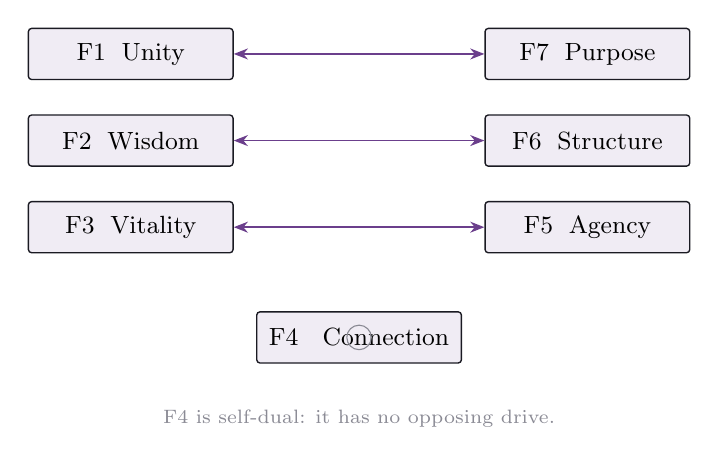
\begin{tikzpicture}
  % Six drives in inversion pairs, F4 self-dual at the centre.
  \foreach \i/\lab/\nm in {0/F1/Unity, 1/F2/Wisdom, 2/F3/Vitality} {
    \node[casnode, minimum width=26mm] (L\i) at (0, -\i*11mm) {\lab \; \nm};
  }
  \foreach \i/\lab/\nm in {0/F7/Purpose, 1/F6/Structure, 2/F5/Agency} {
    \node[casnode, minimum width=26mm] (R\i) at (58mm, -\i*11mm) {\lab \; \nm};
  }
  \foreach \i in {0,1,2} { \draw[casinvol] (L\i) -- (R\i); }
  \node[casnode, minimum width=26mm] (F4) at (29mm, -36mm) {F4 \; Connection};
  \node[draw=casmuted, circle, inner sep=1.1mm, line width=0.4pt] at (F4) {};
  \node[caslabel, anchor=north] at (29mm, -44mm)
    {F4 is self-dual: it has no opposing drive.};
\end{tikzpicture}

\end{document}
